\documentclass[tikz]{standalone}

\IfStandalone{\usepackage{mathtools}}{}


\usetikzlibrary{shapes}
\usetikzlibrary{calc} 
\usetikzlibrary{positioning}
\usetikzlibrary{arrows.meta} 

\providecommand\enpos[2]{\underset{\footnotesize\mathclap{\langle #1,#2 \rangle}}{N}}


% This bascially automates a \newcommand{<name>}{} to ensure
% that a command with the given <name> does not already exist
\providecommand*{\pgfmathsetnewmacro}[2]{%
    \newcommand*{#1}{}% Error if already defined
    \pgfmathsetmacro{#1}{#2}%
}%


\begin{document}
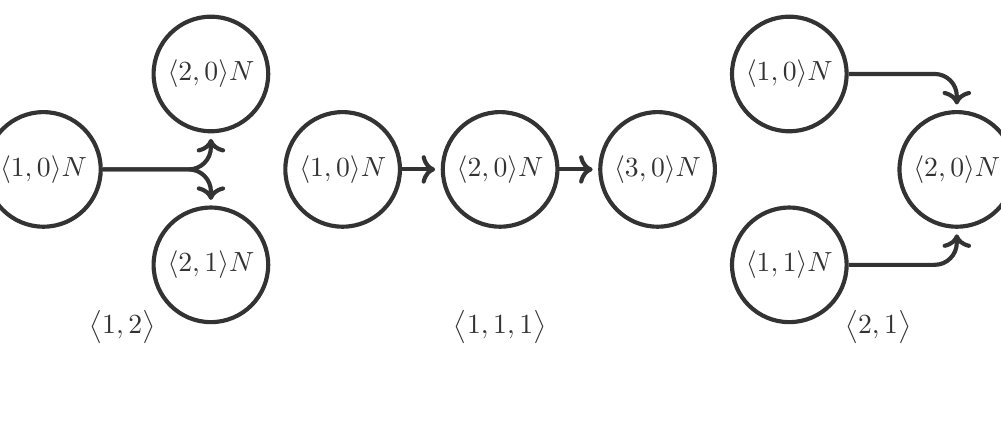
\begin{tikzpicture}[black!80, line width = 1.5pt,
        rounded corners = 8pt,
        shorten >=2pt,]
    \pgfmathsetnewmacro{\bb}{3}
    \useasboundingbox[] (-\bb*2,-\bb) rectangle (\bb*2,\bb*0.6);


    \coordinate (O) at (0,0);

    %\draw[help lines, opacity = 0.1] (-4,-4) grid (4,4);

    \begin{scope}[on grid, xshift = -5.8cm]
        
        \node (O) at (0,0) [circle, draw, fill = white] {$\enpos{1}{0}$};
              
        \node (N1) [circle, draw, fill = white, above right=1.5 of O.south east, yshift = 1ex] {$\enpos{2}{0}$};
        \node (N2) [circle, draw, fill = white, below right=1.5 of O.north east, yshift = -1ex] {$\enpos{2}{1}$};

        \draw[->] (O) -| (N1);
        \draw[->] (O) -| (N2);


        \node (notation1) [below right = of O, yshift = -1cm ] {$\big\langle 1,2 \big\rangle$};
    \end{scope}
        
    \begin{scope}[on grid, xshift = +5.8cm]
        
        \node (O) at (0,0) [circle, draw, fill = white] {$\enpos{2}{0}$};
              
        \node (N1) [circle, draw, fill = white, above left=1.5 of O.south west, yshift = 1ex] {$\enpos{1}{0}$};
        \node (N2) [circle, draw, fill = white, below left=1.5 of O.north west, yshift = -1ex] {$\enpos{1}{1}$};

        \draw[->] (N1) -| (O);
        \draw[->] (N2) -| (O);

        \node (notation1) [below left = of O, yshift = -1cm ] {$\big\langle 2,1 \big\rangle$};
    \end{scope}

    
    \begin{scope}[on grid]
        
        \node (O) at (0,0) [circle, draw, fill = white] {$\enpos{2}{0}$};
              
        \node (N1) [circle, draw, fill = white, left=2 of O] {$\enpos{1}{0}$};
        \node (N2) [circle, draw, fill = white, right=2 of O] {$\enpos{3}{0}$};

        \draw[->] (N1) -- (O);
        \draw[->] (O) -- (N2);
        
        \node (notation1) [below = of O, yshift = -1cm ] {$\big\langle 1,1,1 \big\rangle$};
    \end{scope}
    
    
    
\end{tikzpicture}
\end{document}